\documentclass[11pt,letterpaper]{article}
\usepackage[T1]{fontenc}
\usepackage[utf8]{inputenc}
\usepackage{lmodern}
\usepackage{microtype}
\usepackage{geometry}
\geometry{left=0.88in,right=0.88in,top=0.93in,bottom=0.88in,headheight=23pt,headsep=16pt,footskip=27pt}
\usepackage{amsmath,amssymb,amsthm,mathtools,mathrsfs}
\usepackage{array,booktabs,tabularx}
\usepackage[dvipsnames]{xcolor}
\usepackage{fancyhdr,titlesec,needspace}
\usepackage{tikz}
\usetikzlibrary{arrows.meta,decorations.pathreplacing,calc}
\usepackage[colorlinks=true,urlcolor=tealblue,linkcolor=tealblue,citecolor=tealblue]{hyperref}
\definecolor{ink}{HTML}{1F2A33}
\definecolor{tealblue}{HTML}{226A73}
\definecolor{muted}{HTML}{65747E}
\definecolor{lightline}{HTML}{C5D1D3}
\definecolor{soft}{HTML}{F3F7F6}
\definecolor{warm}{HTML}{A46E44}
\hypersetup{pdftitle={The 3 Body Mirror: Exact Return, Fibonacci Conjugacy, and the Nonlinear Boundary},pdfauthor={Anthony Vito Coppa},pdfsubject={Newtonian three-body dynamics, reversing symmetry, analytic branch conjugacy, Birkhoff normal form}}
\setlength{\parindent}{0pt}
\setlength{\parskip}{0.54em}
\setlength{\emergencystretch}{3em}
\allowdisplaybreaks[1]
\pagestyle{fancy}
\fancyhf{}
\fancyhead[L]{\footnotesize\sffamily\textcolor{muted}{THE 3 BODY MIRROR}}
\fancyhead[R]{\footnotesize\sffamily\textcolor{muted}{COPPALINI ARCHITECTURE}}
\fancyfoot[C]{\footnotesize\sffamily\textcolor{muted}{\thepage}}
\renewcommand{\headrulewidth}{0.35pt}
\renewcommand{\headrule}{\hbox to\headwidth{\textcolor{lightline}{\leaders\hrule height \headrulewidth\hfill}}}
\titleformat{\section}{\Large\bfseries\color{ink}}{\thesection.}{0.6em}{}
\titleformat{\subsection}{\large\bfseries\color{tealblue}}{\thesubsection.}{0.55em}{}
\titlespacing*{\section}{0pt}{1.4em}{0.5em}
\titlespacing*{\subsection}{0pt}{1.1em}{0.4em}
\newtheoremstyle{paper}{0.7em}{0.7em}{\normalfont}{} {\bfseries\color{tealblue}}{.}{0.5em}{}
\theoremstyle{paper}
\newtheorem{theorem}{Theorem}
\newtheorem{proposition}{Proposition}
\newtheorem{corollary}{Corollary}
\newtheorem{lemma}{Lemma}
\newtheorem{remark}{Remark}
\renewcommand{\qedsymbol}{$\square$}
\newcommand{\GN}{\mathsf G_{\!N}}
\newcommand{\Flow}{\Phi}
\newcommand{\Rvs}{\mathscr R}
\newcommand{\euler}{\mathsf E}
\newcommand{\wt}[1]{\textcolor{tealblue}{#1}}
\newcommand{\term}[1]{\textbf{#1}}
\begin{document}

\hypersetup{pageanchor=false}
\begin{titlepage}
\thispagestyle{empty}
\vspace*{0.42in}
{\color{tealblue}\rule{\textwidth}{1.45pt}}\par
\vspace{0.38in}
{\sffamily\footnotesize\bfseries\color{tealblue} COPPALINI ARCHITECTURE\enspace/\enspace MATHEMATICAL PHYSICS}\par
\vspace{0.29in}
{\fontsize{33}{37}\selectfont\bfseries\color{ink}The 3 Body\\[0.06em]Mirror\par}
\vspace{0.19in}
{\Large\color{tealblue}Exact Return, Fibonacci Conjugacy,\\[0.13em]and the Nonlinear Boundary\par}
\vspace{0.24in}
{\color{lightline}\rule{\textwidth}{0.6pt}}
\vspace{0.30in}
\begin{minipage}{0.97\textwidth}
\large\color{ink}
A moving observer can recover the relative configuration of a three-body system from within it. Newtonian reflection and time reversal supply an exact inverse; a selected hyperbolic sector of the equal-mass Euler orbit realizes the Fibonacci transport $Q^2$. The nonlinear system preserves the mirror relation, while its fourth-order normal form determines where linear conjugacy stops.
\end{minipage}
\vfill
\begin{center}
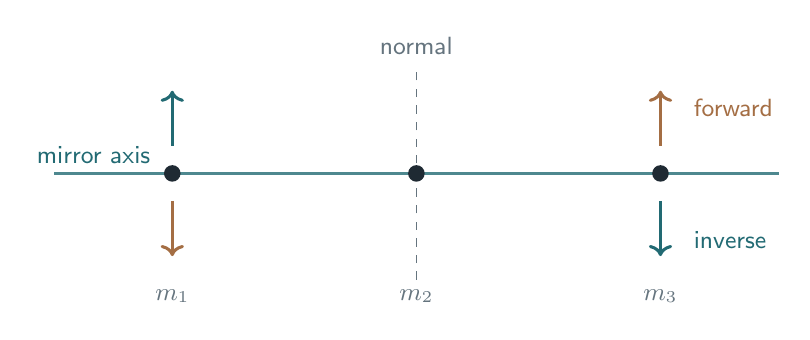
\begin{tikzpicture}[scale=1.0, every node/.style={font=\small\sffamily}]
  \draw[very thick,tealblue!80] (-4.6,0) -- (4.6,0);
  \draw[dashed,muted] (0,-1.35) -- (0,1.35);
  \fill[ink] (-3.1,0) circle(0.105);
  \fill[ink] (0,0) circle(0.105);
  \fill[ink] (3.1,0) circle(0.105);
  \draw[->,line width=1.1pt,warm] (-3.1,-0.35) -- (-3.1,-1.05);
  \draw[->,line width=1.1pt,warm] (3.1,0.35) -- (3.1,1.05);
  \draw[->,line width=1.1pt,tealblue] (-3.1,0.35) -- (-3.1,1.05);
  \draw[->,line width=1.1pt,tealblue] (3.1,-0.35) -- (3.1,-1.05);
  \node[muted,above] at (0,1.39) {normal};
  \node[tealblue,above] at (-4.1,0.0) {mirror axis};
  \node[muted,below] at (-3.1,-1.35) {$m_1$};
  \node[muted,below] at (0,-1.35) {$m_2$};
  \node[muted,below] at (3.1,-1.35) {$m_3$};
  \node[warm,right] at (3.4,0.83) {forward};
  \node[tealblue,right] at (3.4,-0.84) {inverse};
\end{tikzpicture}
\end{center}
\vfill
\begin{tabularx}{\textwidth}{@{}lX@{}}
\textsc{Author} & Anthony Vito Coppa \\
\textsc{Date} & 7 November 2026 \\
\textsc{Status} & Manuscript draft for mathematical review \\
\textsc{Supporting computation} & Two independently implemented SymPy checks; provenance disclosed
\end{tabularx}
\vspace{0.31in}
{\color{tealblue}\rule{\textwidth}{1.45pt}}
\end{titlepage}
\hypersetup{pageanchor=true}

\section*{Abstract}
We give an explicit realization of a mirror--return structure in the planar Newtonian three-body problem. With known masses and complete relative-position vectors in a common oriented frame, an observer reconstructs the barycentric configuration without knowing their own translational trajectory. An orthogonal reflection, composed with time reversal, is a reversing symmetry of the full collision-free flow. For the equal-mass Euler collinear relative equilibrium, a two-dimensional hyperbolic variational sector is conjugate, at a declared sampling interval, to $Q^2$ for the Fibonacci matrix $Q=\bigl(\begin{smallmatrix}1&1\\1&0\end{smallmatrix}\bigr)$, with the gravitational reversor corresponding to an exact root mirror $H$. The one-dimensional local strong stable and unstable manifolds admit compatible analytic linearizations: their union carries a nonlinear conjugacy to $Q^2$ on its two eigenlines. The fourth-order Birkhoff coefficient is evaluated exactly and independently verified to be nonzero, obstructing formal and smooth linearization beyond that cross in the specified local saddle dynamics. The result supplies an exact physical witness, with an explicit boundary; it does not assert a general closed-form solution of the three-body problem or an astronomically selected Fibonacci period.

\section{The ordinary physical statement}

A person moving with a system can still locate its parts relative to one another. The origin of observation moves; the differences remain available. A mirror can exchange orientations without changing gravitational distances. Run a reflected trajectory backward, and Newton's equations admit it as an exact solution.

Near one classical rotating three-body orbit, small differences grow and shrink along two distinguished directions. At a chosen interval those factors are the two Fibonacci eigenvalues $\varphi^2$ and $\varphi^{-2}$. This identification is exact for the linearized motion and, after a local change of coordinates, exact along the nonlinear stable and unstable branches. A separately calculated fourth-order coefficient shows why the same linear description cannot be extended without changing the dynamics.

The governing question is therefore concrete: \emph{what does the mirror preserve, what does the chosen reader resolve, and where does the exact agreement stop?}

\section{Interior reference and barycentric reconstruction}

Let the positions of three positive masses be $r_i(t)\in\mathbb R^2$, and let an observer occupy $h(t)\in\mathbb R^2$. Suppose the masses $m_i>0$ are known and the observer reads simultaneous relative vectors in a common oriented frame:
\begin{equation}
q_i=r_i-h,\qquad M=\sum_{i=1}^3m_i,\qquad \bar q=\frac{1}{M}\sum_i m_iq_i.
\label{eq:inside}
\end{equation}

\begin{proposition}[Interior-to-barycentric identity]
If $R_{\rm CM}=M^{-1}\sum_i m_i r_i$, then
\begin{equation}
\boxed{q_i-\bar q=r_i-R_{\rm CM}.}
\label{eq:bary}
\end{equation}
\end{proposition}
\begin{proof}
Equation \eqref{eq:inside} gives $\bar q=R_{\rm CM}-h$. Subtracting yields \eqref{eq:bary}. The observer trajectory cancels, including any translational acceleration.
\end{proof}

The reconstructed configuration is centered at the three-body barycenter. Absolute translation and global orientation are gauge choices unless separately fixed by measured data. The identity concerns the classical relative configuration; it imposes no constraint on an observer's consciousness or biological state.

\section{Newtonian mirror and the root metric}

Write $\GN$ for Newton's constant. The collision-free planar equations are
\begin{equation}
\ddot r_i=\GN\sum_{j\ne i}m_j\frac{r_j-r_i}{\|r_j-r_i\|^3},\qquad i=1,2,3.
\label{eq:newton}
\end{equation}

For every planar orthogonal matrix $D$, relative distances are preserved. Hence, if $r_i(t)$ solves \eqref{eq:newton}, so does $D r_i(-t)$. On phase space the operation
\begin{equation}
\Rvs_D(r,p)=(Dr,-Dp)
\quad\text{satisfies}\quad
\boxed{\Rvs_D\Flow_t=\Flow_{-t}\Rvs_D,}
\label{eq:reversor}
\end{equation}
where $\Flow_t$ denotes Newtonian evolution on its collision-free domain.

Now fix the exact two-dimensional root:
\begin{equation}
Q=\begin{pmatrix}1&1\\1&0\end{pmatrix},\qquad
\Omega=\begin{pmatrix}0&1\\-1&0\end{pmatrix},\qquad
G=[Q,\Omega]=\begin{pmatrix}-2&1\\1&2\end{pmatrix},
\label{eq:root}
\end{equation}
\begin{equation}
H=\frac{G}{\sqrt5},\qquad
S=\Omega H=\frac{2Q-I}{\sqrt5},\qquad
\varphi=\frac{1+\sqrt5}{2}.
\label{eq:operators}
\end{equation}

Direct multiplication verifies
\begin{align}
H^2=S^2&=I, & H^TH=S^TS&=I, & \det H=\det S&=-1, \label{eq:orth}\\
H^TGH&=G, & S^TGS&=-G, & HSH&=-S, \label{eq:metric}\\
Q^2&=e^{2(\log\varphi)S}, && HQ^2H=(Q^2)^{-1}.\label{eq:gold}
\end{align}

These give two separately typed facts. Both $H$ and $S$ are \emph{Euclidean isometries}, so they take Newtonian solutions to solutions. The auxiliary split form $G$ is preserved by $H$ and sign-reversed by $S$. Thus the ``metric flip'' in \eqref{eq:metric} is a precise statement about the root's signature-$(1,1)$ form, not an inversion of the positive Euclidean distance used by gravity.

The matrix $Q$ itself has determinant $-1$ and cannot be the positive-time map of a continuous real planar flow. Its square has determinant $+1$, and \eqref{eq:gold} displays a real flow realization. The choice of $Q^2$ therefore has a structural, rather than merely notational, role.

\section{An exact Euler three-body witness}

Choose equal masses $m>0$. Let $e_H=(1,\varphi^3)/\sqrt{10+4\sqrt5}$ be the unit $+1$ eigenaxis of $H$ (distinct from the $Q^2$ eigenvector $u_+$ below), and set
\begin{equation}
r_1(0)=-ae_H,\qquad r_2(0)=0,\qquad r_3(0)=ae_H,\qquad a>0.
\end{equation}
In an orthonormal frame aligned with $e_H$ these positions are $(-a,0)$, $(0,0)$, and $(a,0)$.
The positions
\begin{equation}
\boxed{r_i(t)=R(\omega t)r_i(0),\qquad
\omega^2=\frac{5\GN m}{4a^3}}
\label{eq:euler}
\end{equation}
solve \eqref{eq:newton}. The middle body's net force is zero; each outer body feels $\GN m/a^2+\GN m/(2a)^2=5\GN m/(4a^2)$ toward the center, exactly the centripetal force required by \eqref{eq:euler}. This is the equal-mass Euler collinear relative equilibrium \cite{broucke,yamada}. Direct calculation verifies $He_H=e_H$; this physical mirror axis differs from the Fibonacci eigenvectors exchanged by $H$ in \eqref{eq:modes}.

The specified $H$ is the reflection through the initial line. For any planar rotation $R(\alpha)$,
\begin{equation}
HR(-\alpha)=R(\alpha)H,
\qquad\text{hence}\qquad
\boxed{Hr_i(-t)=r_i(t).}
\label{eq:eulermirror}
\end{equation}
The full nonlinear orbit therefore has an exact physical mirror inverse. In the corotating, rotation-reduced coordinates, the orbit is an equilibrium $\euler$ fixed by the reversing operation.

\section{Linearized transport and Fibonacci conjugacy}

Set $m=a=1$ and $\GN=4/5$. Then $\omega=1$ and the total angular momentum is $\ell=2$. Jacobi reduction of translation and rotation, at fixed $\ell$, gives canonical variables $(r,x,y;p,u,v)$ with Hamiltonian
\begin{align}
\mathcal H={}&\frac{p^2+u^2+v^2}{2}+\frac{(2-xv+yu)^2}{2r^2} \notag\\
&-\frac45\left(\frac1{\sqrt2r}+
\frac{\sqrt2}{\sqrt{(r-\sqrt3x)^2+3y^2}}+
\frac{\sqrt2}{\sqrt{(r+\sqrt3x)^2+3y^2}}\right).
\label{eq:ham}
\end{align}

The Euler equilibrium is $\euler=(\sqrt2,0,0;0,0,0)$. Writing $\rho=r-\sqrt2$, the quadratic Hamiltonian is
\begin{equation}
\mathcal H_2=\frac{p^2+\rho^2+u^2+v^2}{2}+uy-vx-\frac{12}{5}x^2+\frac65y^2.
\label{eq:quad}
\end{equation}
Its Hamiltonian linearization has characteristic polynomial
\begin{equation}
\det(\lambda I-A_6)=(\lambda^2+1)(\lambda^2-\nu^2)(\lambda^2+\kappa^2),
\quad
\nu^2=\frac{1+2\sqrt{51}}5,\quad
\kappa^2=\frac{2\sqrt{51}-1}5.
\label{eq:spec}
\end{equation}

The six-dimensional phase space thus contains one hyperbolic pair $\pm\nu$ and two elliptic pairs $\pm i$, $\pm i\kappa$. Related normal-form analyses of saddle--center--center equilibria appear for the restricted three-body model \cite{jorba}; the present calculation uses three finite equal masses. In the four-dimensional shape subsystem, which contains the hyperbolic two-plane, use $(x,y,x',y')$ as coordinates. Its generator and reversor are
\begin{equation}
A_h=\begin{pmatrix}
0&0&1&0\\0&0&0&1\\29/5&0&0&2\\0&-7/5&-2&0
\end{pmatrix},
\quad
\Rvs_h=\operatorname{diag}(1,-1,-1,1).
\label{eq:Ah}
\end{equation}

Define
\begin{equation}
b=\frac{\sqrt{51}-14}{5\nu},\quad
w_+=\begin{pmatrix}1\\b\\\nu\\\nu b\end{pmatrix},\quad
w_-=\Rvs_hw_+,
\quad
u_+=\begin{pmatrix}\varphi\\1\end{pmatrix},\quad
u_-=Hu_+=\begin{pmatrix}-1\\\varphi\end{pmatrix}.
\label{eq:modes}
\end{equation}
Direct calculation gives
\begin{equation}
A_hw_\pm=\pm\nu w_\pm,
\qquad Q^2u_\pm=\varphi^{\pm2}u_\pm.
\end{equation}

\begin{theorem}[Exact linear physical conjugacy]
Let $W=\operatorname{span}\{w_+,w_-\}$ and set
\begin{equation}
\sigma_* =\frac{2\log\varphi}{\nu}=0.550489470050798\ldots,
\qquad
C=[w_+\ \ w_-]\,[u_+\ \ u_-]^{-1}.
\label{eq:C}
\end{equation}
Then $C:\mathbb R^2\to W$ is an isomorphism and
\begin{equation}
\boxed{e^{A_h\sigma_*}C=CQ^2,\qquad \Rvs_h C=CH.}
\label{eq:intertwine}
\end{equation}
\end{theorem}
\begin{proof}
The vectors $u_\pm$ form an eigenbasis of $Q^2$ with eigenvalues $\varphi^{\pm2}$; the vectors $w_\pm$ form an eigenbasis of $A_h$ with eigenvalues $\pm\nu$. By \eqref{eq:C}, $e^{\pm\nu\sigma_*}=\varphi^{\pm2}$. The first intertwining identity follows on both basis vectors. Both $H$ and $\Rvs_h$ exchange their respective $+$ and $-$ vectors, giving the second identity.
\end{proof}

The interval $\sigma_*$ is \emph{declared from the growth rate}; no astronomical clock has been shown to select it. More generally, every reversible two-dimensional real hyperbolic sector with rate $\nu>0$ and a reversor exchanging the eigenlines admits the same $Q^2$ conjugacy at the chosen interval $2\log\varphi/\nu$, after compatible scaling of eigenvectors. In general units the physical time is $t_*=\sigma_*/\omega$.

\section{The nonlinear cross theorem}

For the reduced Hamiltonian, the reversing involution is
\begin{equation}
\Rvs(r,x,y,p,u,v)=(r,x,-y,-p,-u,v).
\label{eq:reducedR}
\end{equation}
It is anti-symplectic, fixes $\euler$, preserves $\mathcal H$, and obeys \eqref{eq:reversor}. The equilibrium has one-dimensional local analytic strong stable and strong unstable manifolds $W^s_{\rm loc}$ and $W^u_{\rm loc}$, exchanged by $\Rvs$.

\begin{lemma}[Nonlinear mirror conjugacy on the cross]
Let $P=\Flow_{\sigma_*}$ be the time-$\sigma_*$ map of the full reduced Hamiltonian near $\euler$. There are analytic local parametrizations $\chi_+,\chi_-$ of $W^u_{\rm loc},W^s_{\rm loc}$ with
\begin{equation}
\begin{aligned}
P\chi_+(s)&=\chi_+(\varphi^2s), &
P\chi_-(s)&=\chi_-(\varphi^{-2}s),\\
\Rvs\chi_+(s)&=\chi_-(s).&&
\end{aligned}
\label{eq:cross}
\end{equation}
Consequently, $P$ on the union $W^u_{\rm loc}\cup W^s_{\rm loc}$ is analytically conjugate, branch by branch and compatibly with the mirror, to $Q^2$ on its two eigenlines.
\end{lemma}
\begin{proof}
The vector field in \eqref{eq:ham} is analytic near the collision-free equilibrium, and its single expanding and contracting real eigenvalues are nonzero. The local strong invariant branches are analytic. The one-dimensional analytic time map on the expanding branch has multiplier $\varphi^2$; Koenigs linearization, or its real-analytic restriction, supplies $\chi_+$ \cite{milnor}. Set $\chi_-=\Rvs\chi_+$. The reversing relation yields
$P\chi_-=\Rvs P^{-1}\chi_+=\chi_-(\varphi^{-2}s)$.
Identifying the two branch parameters with the root eigenlines $\mathbb Ru_+$ and $\mathbb Ru_-$ completes the conjugacy wherever the local charts are defined.
\end{proof}

The \term{cross} is the union of two one-dimensional invariant branches meeting at $\euler$. This is a local consequence of the analytic stable-manifold and one-dimensional Koenigs linearization theorems, together with the reversor. Its scope is branchwise, rather than a two-dimensional analytic neighborhood. It does not identify the entire six-dimensional neighborhood with a two-dimensional linear map.

\section{The fourth-order stopping condition}

Let $\{\xi,\eta\}=1$ be a canonically normalized hyperbolic eigenpair, and let $I=\xi\eta$. The Birkhoff normal form of \eqref{eq:ham}, including the contributions from both center modes, contains
\begin{equation}
\mathcal H_{\rm NF}=\mathcal H(\euler)+\nu I+\text{center terms}+a I^2+\text{other higher terms}.
\label{eq:nf}
\end{equation}
The coefficient $a$ is the pure hyperbolic resonant coefficient at degree four.

The cubic Hamiltonian, with $\rho=r-\sqrt2$, has the exact form
\begin{equation}
\mathcal H_3=\frac{\sqrt2\rho}{10}
\bigl(-5\rho^2-10uy+10vx+36x^2-18y^2\bigr).
\label{eq:cubic}
\end{equation}
The quartic coefficient of $I^2$ receives both a direct term from $\mathcal H_4$ and the contribution of the canonical Lie transform removing $\mathcal H_3$. Independently implemented symbolic and full six-dimensional Taylor-tensor methods agree:
\begin{align}
 a_{\rm direct}&=-1.547622997565423\ldots,\notag\\
 a_{\rm cubic}&=-1.225471490664213\ldots,\notag\\
 \boxed{a}&=\boxed{-\frac{82891803+215881566\sqrt{51}}{585841760}}
 =-2.773094488229637\ldots.
\label{eq:a}
\end{align}

For the time-$\sigma$ map, $\dot\xi=(\nu+2aI)\xi+\cdots$ and $\dot\eta=-(\nu+2aI)\eta+\cdots$. Thus its first pure hyperbolic resonant coefficient is
\begin{equation}
\boxed{c_1(\sigma)=2\sigma a\ne0\quad\text{for every }\sigma>0.}
\label{eq:c1}
\end{equation}
At the declared Fibonacci sampling time,
\begin{equation}
\boxed{c_1(\sigma_*)=-3.053118630452643\ldots.}
\end{equation}

\begin{corollary}[First resonant obstruction for the sampled map]
For the time-$\sigma_*$ map $P$ of the fixed-angular-momentum reduced Hamiltonian, $c_1(\sigma_*)\ne0$ is the first cubic resonant coefficient in its hyperbolic component. Therefore $P$ is not formally conjugate to its full linear map on an open neighborhood by a near-identity time-preserving change of coordinates. Analytic and $C^\infty$ linearizations of this type are likewise obstructed. The analytic conjugacy on the stable/unstable cross remains exact.
\end{corollary}
\begin{proof}
The quartic term $aI^2$ in the Hamiltonian produces the cubic resonant monomial $2a\xi^2\eta$ in the hyperbolic vector field and coefficient $2\sigma_*a$ in the sampled map, after factoring out the linear multiplier. The six eigenvalues of $DP(\euler)$ are $e^{\pm\nu\sigma_*}$, $e^{\pm i\sigma_*}$, and $e^{\pm i\kappa\sigma_*}$. There are no quadratic resonances. For degree-three monomials, a new discrete-time alias resonance would require a center-frequency difference to be an integer multiple of $2\pi/\sigma_*$. Every candidate frequency difference has absolute value at most $4\kappa$; since $4\kappa\sigma_*<2\pi$, all degree-three map resonances are already continuous-time resonances. In particular, the nonzero pure-hyperbolic term $\xi^2\eta$ cannot be removed by a formal near-identity change. Any analytic or $C^\infty$ linearization induces a formal one. On either branch of the cross $I=0$, so the branchwise result in \eqref{eq:cross} remains exact.
\end{proof}

\emph{Boundary.} This is a differential/formal obstruction; it is not a claim against topological conjugacy. A claim independent of all choices of nonlinear invariant surfaces, or an extension to the complete Sun--Earth--Moon ephemeris, requires its own theorem and evidence. Since $a\ne0$, higher resonant coefficients are unnecessary to establish the stated failure of smooth linearization.

\section{Independent computational check}

Two independently implemented computational checks accompany the exact coefficient. \texttt{verify\_euler\_}\allowbreak\texttt{birkhoff\_c1.py} was prepared with ChatGPT (OpenAI) assistance in this project; it symbolically expands \eqref{eq:ham} and checks the spectrum, eigenvectors, symplectic normalization, and coefficient. \texttt{audit\_c1.py} was prepared in a separate review with Claude (Anthropic) assistance. It accepts the same reduced Hamiltonian as input, but derives Taylor tensors directly, performs its own generic six-dimensional Lie transform, and independently checks the reduction against the unreduced Newton equations. Their independence concerns the implemented calculations and the raw-equations check, not independent discovery of the starting Hamiltonian.

\begin{center}\small
\begin{tabularx}{\textwidth}{@{}>{\raggedright\arraybackslash}p{0.56\textwidth}>{\raggedleft\arraybackslash}X@{}}
\toprule
\textbf{Check} & \textbf{Observed result}\\
\midrule
$|\mathcal H_{\rm reduced}-E_{N\text{-body}}|$ & $4.44\times10^{-16}$\\
Angular momentum $\ell$ & $2$\\
Max. finite-difference dynamical residual & $1.41\times10^{-9}$\\
Canonical Poisson bracket $\{\xi,\eta\}$ & $1$\\
Hyperbolic rate $\nu$ & $1.748305285531431$\\
Sampling interval $\sigma_*$ & $0.550489470050798$\\
Quartic coefficient $a$ & $-2.773094488229637$\\
First return coefficient $c_1$ & $-3.053118630452643$\\
\bottomrule
\end{tabularx}
\end{center}

The small residuals are numerical consistency checks. The exact expressions and proofs establish the mathematical claims; numerical agreement supplies an independent computational receipt. The accompanying files are \texttt{verify\_euler\_}\allowbreak\texttt{birkhoff\_c1.py} and \texttt{audit\_c1.py}.

\section{Result and scope}

\begin{center}
\setlength{\fboxsep}{11pt}
\fcolorbox{lightline}{soft}{\begin{minipage}{0.89\textwidth}
\textbf{The 3 Body Mirror, in one statement.} From complete interior relative vectors, a moving observer reconstructs a barycentric three-body configuration. Newtonian dynamics admit an exact reflection--time inverse. At the equal-mass Euler relative equilibrium, the sampled hyperbolic variational transport is exactly conjugate to $Q^2$, and the full nonlinear flow carries the same mirror-compatible conjugacy on its one-dimensional stable and unstable cross. A nonzero fourth-order coefficient $a$ witnesses the boundary of formal and smooth linearization beyond that cross.
\end{minipage}}
\end{center}

This construction joins three offices that have different mathematical status: \term{interior reference} is an exact coordinate identity; \term{mirror return} is an exact physical symmetry; \term{Fibonacci transport} is an exact conjugacy on a declared variational sector and nonlinear invariant cross. The computed quartic term marks the first nonlinear limit of that representation.

The construction does not solve arbitrary three-body initial conditions in closed form. Its sampling interval is selected mathematically, rather than measured from celestial periods. An empirical Sun--Earth--Moon realization and a biological phase-entrainment realization each demand their own dynamical model, observables, and comparison data. These are separate continuations of a completed local theorem.

\textbf{Common-sense closure.} The observer moves with the world. Relative differences still supply a reference. The mirror carries a lawful inverse. The nonlinear system decides exactly how far the linear read can travel.

\section*{References and verification}
\begin{thebibliography}{9}\setlength{\itemsep}{0.2em}
\bibitem{broucke} R. Broucke, E. Davoust, J. D. Anderson, H. Lass, and L. Blitzer, ``Periodic solutions about the collinear Lagrangian solution in the general problem of three bodies,'' \emph{Celestial Mechanics} \textbf{24} (1981), 63--82. \href{https://doi.org/10.1007/BF01228794}{doi:10.1007/BF01228794}.
\bibitem{yamada} K. Yamada and H. Asada, ``Collinear solution to the general relativistic three-body problem,'' \emph{Phys. Rev. D} \textbf{82} (2010), 104019, Section I (Newtonian background). \href{https://doi.org/10.1103/PhysRevD.82.104019}{doi:10.1103/PhysRevD.82.104019}; \href{https://arxiv.org/abs/1010.2284}{arXiv:1010.2284}.
\bibitem{milnor} J. Milnor, \emph{Dynamics in One Complex Variable}, 3rd ed., Princeton University Press (2006), Theorem 8.2 (Koenigs linearization).
\bibitem{jorba} A. Jorba and J. Masdemont, ``Dynamics in the center manifold of the collinear points of the restricted three body problem,'' \emph{Physica D} \textbf{132} (1999), 189--213. \href{https://doi.org/10.1016/S0167-2789(99)00042-1}{doi:10.1016/S0167-2789(99)00042-1}. Related normal-form context; a different physical model.
\end{thebibliography}
\end{document}
